% Chapter 1

\chapter{Introduction} % Main chapter title
\label{Chapter1} % For referencing the chapter elsewhere, use \ref{Chapter1} 

\lhead{Chapter 1. \emph{Introduction}} % This is for the header on each page - perhaps a shortened title

%----------------------------------------------------------------------------------------
% Section 1
%----------------------------------------------------------------------------------------

\section{Context}

%-- machine learning in safety-critical systems
\Gls{ml} algorithms are becoming increasingly present in systems that operate within shared environments
with humans, or involve direct interaction with humans themselves~\citep{pereira}. These systems 
are often defined as safety-critical, such that their failures lead to unintended and potentially harmful behaviours~\citep{amodei}.
Examples of these systems include autonomous automotive systems, traffic control systems, medical devices, aviation software,
industrial robotics, and many more cyber-physical systems that interact with our environment.
Many of these systems have so far only existed as proof of concepts, but are steadily approaching commercial use within our society.

%-- prone to adversarial attacks
Additionally, recent research has exposed broad vulnerabilities to adversarial attacks within data driven \gls{ml} algorithms,
including \Glspl{nn}; where applying small but intentional perturbations to an input which are not noticible to humans,
can lead to a model outputting an incorrect classification with high confidence.~\citep{goodfellow}.
An example of such an attack can be seen in \textit{Fig.~\ref{fig:adversarialpatch}}.
Consequently, the testing and verification of \gls{ml} for the use of controlling safety-critical systems has become a focused area of research in recent years.

\begin{figure}[H]
	\centering
        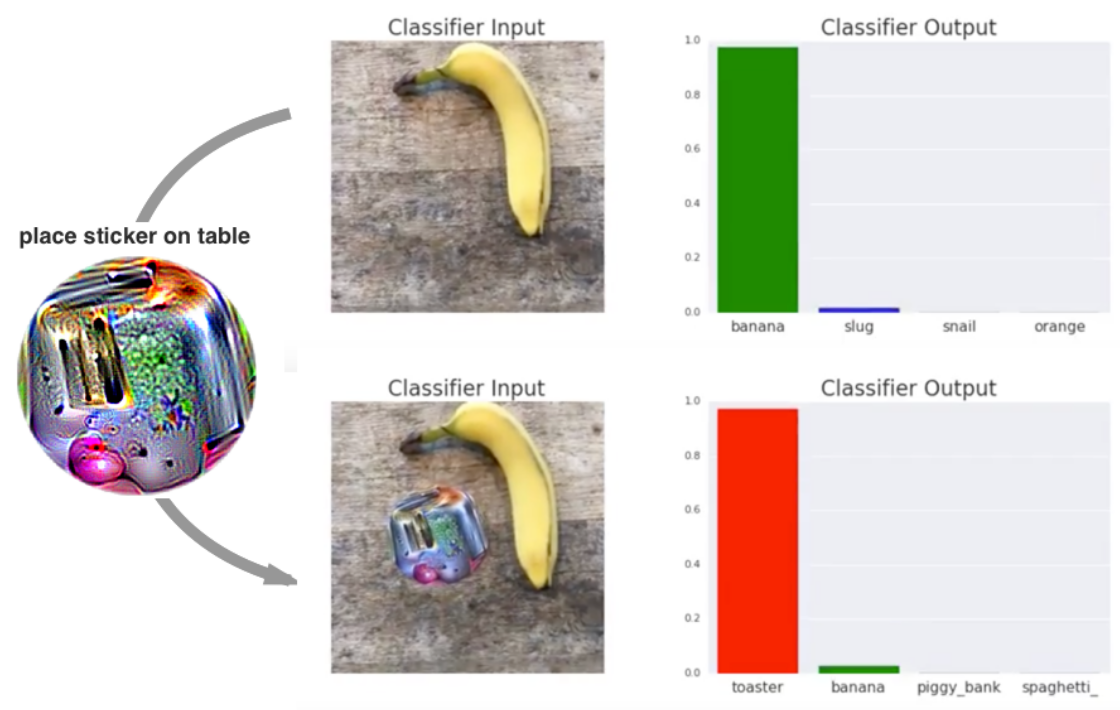
\includegraphics[width=1.0\textwidth]{media/introduction/sticker.png}
        \rule{35em}{0.5pt}
        \caption[Google's Aversarial Patch]{\textbf{Google's Adversarial Patch} -- An example of a method to create targeted adversarial attacks on \glspl{nn} by adding carefully designed noise via a physical patch~\citep{brown2018}.}\label{fig:adversarialpatch}
\end{figure}

%-- definition of software testing and verification
This thesis will use the following definitions for software testing and verification.
Software testing, or validation, is defined as the evaluation of a system under various conditions and observing its behaviour while
looking for defects~\citep{pereira}. In the context of \gls{ml} development, testing is used to
ensure that a trained model generalises accurately to some previously unseen test data.

Verification is defined as the process of determining whether the products of a phase of the software development process fulfill
the requirements established during the previous phase~\citep{ammann2008}. Formal verification in other words, formulates logical arguments
that a system will not act abnormally under a wide range of circumstances, and can be used to determine not only generality, but also the robustness and correctness of a system.

%-- challenges when verifying ML systems
The challenges regarding verification of \gls{ml} models stem from the typically less deterministic and more statistically-oriented nature of their algorithms, which
lead to a lower degree of understanding than software that is explicitly programmed to perform a specific task~\citep{bishop}. These types of systems are
commonly referred to as \textit{black box} systems, where the internal mechanisms are not revealed; in other words, it is impossible to understand a model just by
looking at its parameters~\citep{molnar2019}.


%----------------------------------------------------------------------------------------
% Section 2
%----------------------------------------------------------------------------------------
\section{Motivation}

Public calls for \textit{sensible} or \textit{verifiable \Gls{ai}} have been raised in recent years due to ever increasing
development of complex and pervasive systems that are entering into our everyday lives~\citep{russell2016}.
Although there have been advances in research concerned with the verification of \Glspl{mas}~\citep{lomuscio2017, kouvaros2016},
there has until recently been very little work in the area of formally verifying \gls{ml} algorithms.

%-- lack of verification tools across different languages used for ML
%-- python, although the most popular pl for ml, is dynamically typed, causing challenges for formal verification
%-- languages typically used within ML communities are not designed, or have lack of developed verification tools

%----------------------------------------------------------------------------------------
% Section 3
%----------------------------------------------------------------------------------------
\section{Aims \& Objectives}
